%\documentclass[aps,prd,nofootinbib]{revtex4-1}
\documentclass[singlepage,notitlepage,nofootinbib,11pt]{revtex4-1}
\usepackage{amsmath}
\usepackage{graphicx}
\usepackage{subfig}
\usepackage{epsfig}
\usepackage{listings}
\usepackage[hidelinks,hyperfootnotes=false,bookmarks=false,colorlinks=true]{hyperref}
\begin{document}
\title{Problem Set 2 - G6080}
\author{Victor Genty}
\email{vgenty@nevis.columbia.edu}
\homepage{www.nevis.columbia.edu/~vgenty}
%\affiliation{Department of Physics, Duke University, Durham, NC 27707, USA}
\date{\today}
\begin{abstract}
\centering
Source code can be found at \href{https://github.com/vgenty/G6080/tree/master/ps2}{github.com/vgenty/G6080/ps2}
\end{abstract}
\maketitle
\section{Problem 1 - Planets}
\subsection{Part 1}
The lowest order corrector-predictor method is implemented in Python with the NumPy library to evolve the N body equations of motion. Using the initial conditions specified in Part 1, we find that a step size ``\verb|p.dx|'' of roughly $\mathbf{10^{-4}}$ with $\mathbf{300}\text{\bf{,}}\mathbf{000}$ steps was sufficient to keep the energy from deviating either above or below it's initial energy by one percent.
\begin{figure}[h]
  \centering
  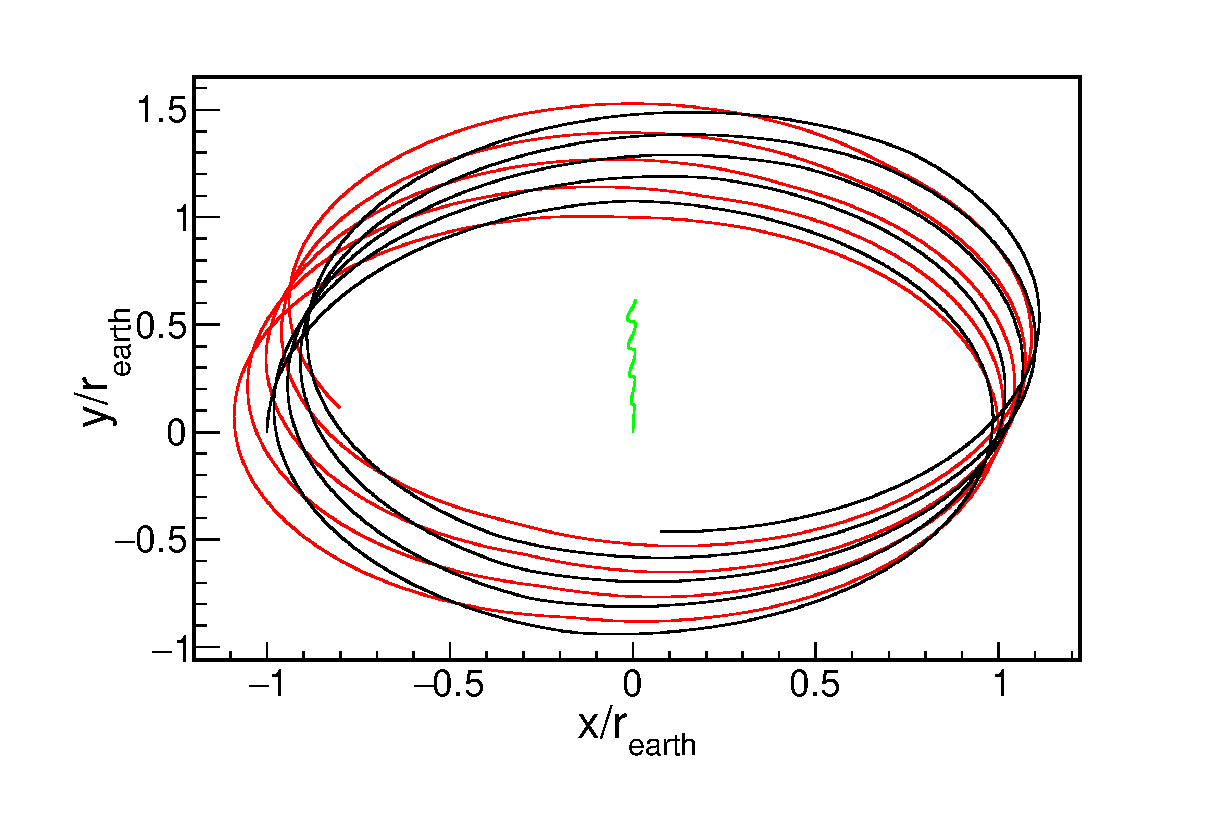
\includegraphics[width=0.5\textwidth]{figures/1r.eps}
  \subfloat[][]{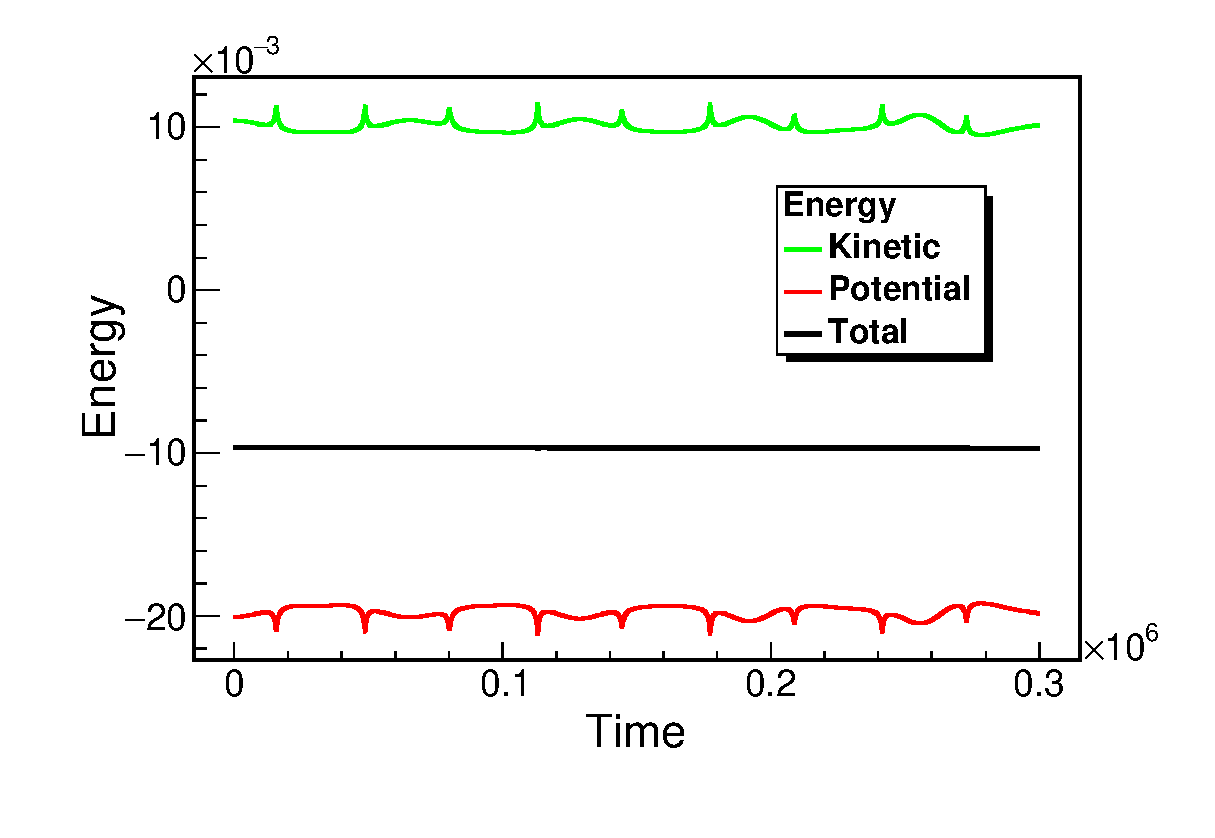
\includegraphics[width=0.5\textwidth]{figures/1es.eps}}
  \subfloat[][]{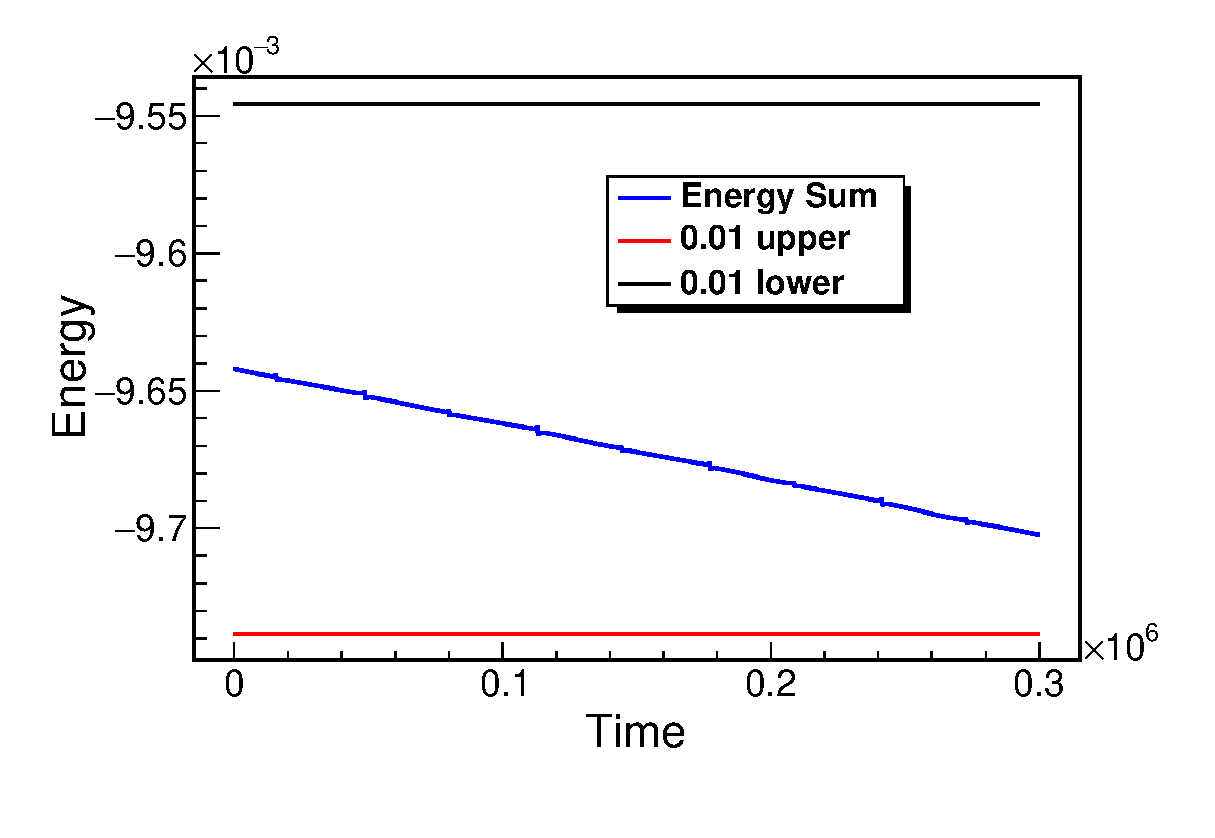
\includegraphics[width=0.5\textwidth]{figures/1ee.eps}}\\
\hfill
  \caption{\label{fig1} Plots for Part 1. Top pane are the coordinate locations of the three planets the green, red, and black lines represent the trajectories of the sun and two orbiting planets. The bottom left pane shows the total kinetic and potential energies. The bottom right shows the deviation of the total energy as a function of time. The lines above and below represent 1\% bounds on the initial total energy.}
\end{figure}
The trajectory, kinetic, potential, and total energy are plotted in Fig. \ref{fig1}.
\subsection{Part 2}
With the initial conditions specified in Part 2 and a step size of 60,000, the predictor-corrector algorithm fails for short range interactions shown in Fig. \ref{fig2}.
\begin{figure}[h]
  \centering
  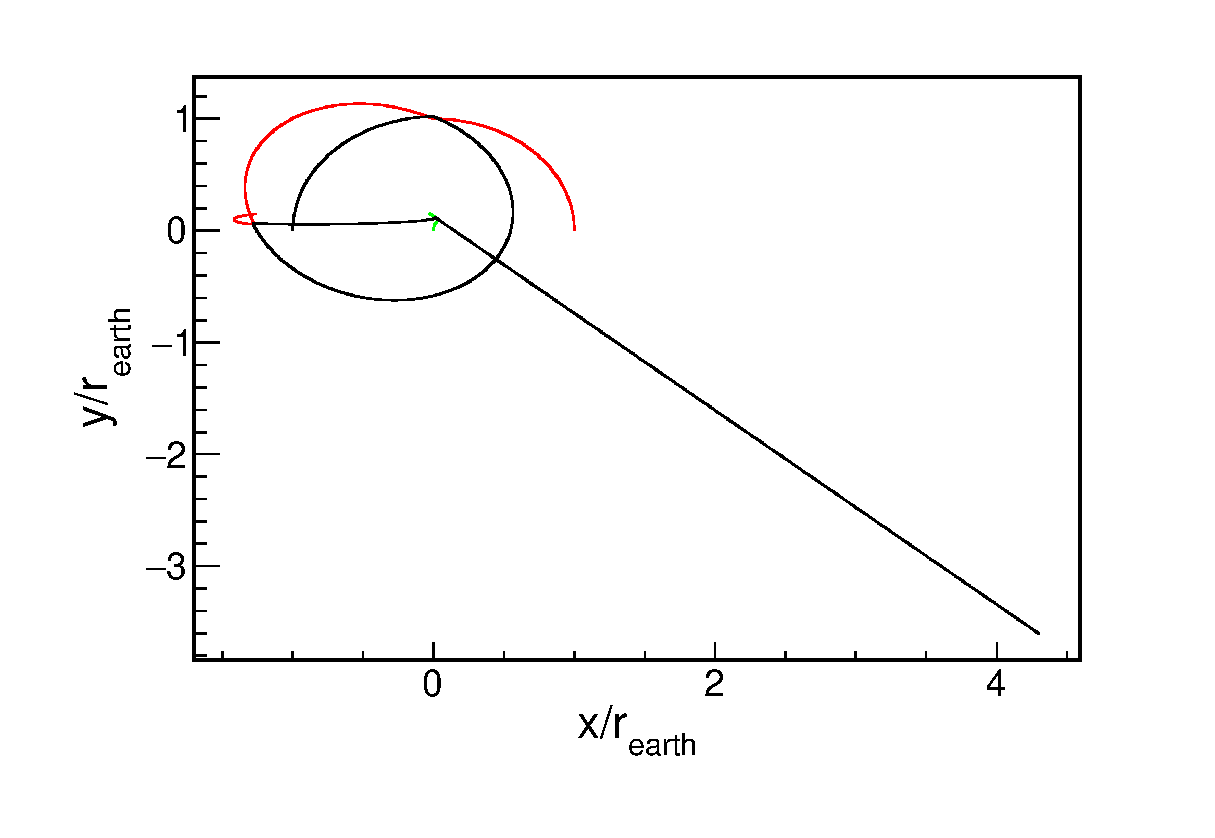
\includegraphics[width=0.5\textwidth]{figures/2r.eps}
  \subfloat[][]{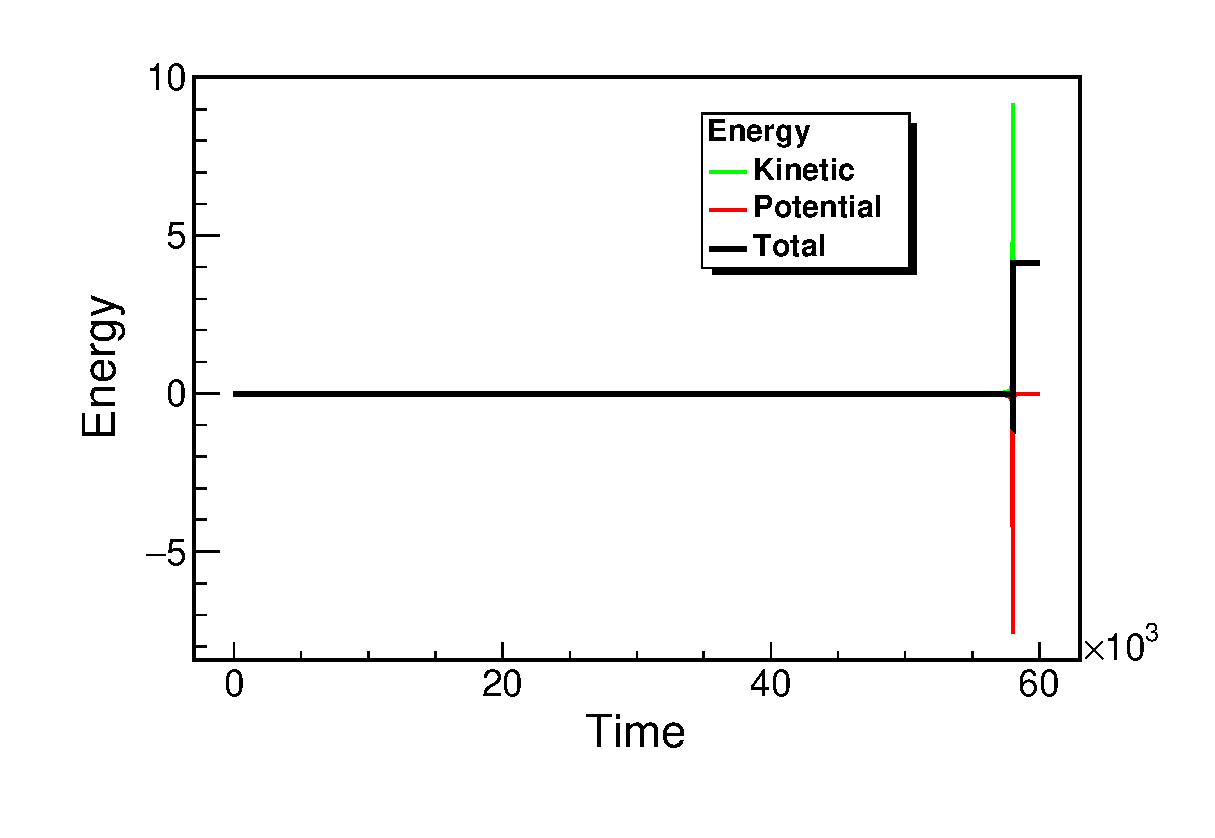
\includegraphics[width=0.5\textwidth]{figures/2es.eps}}
  \subfloat[][]{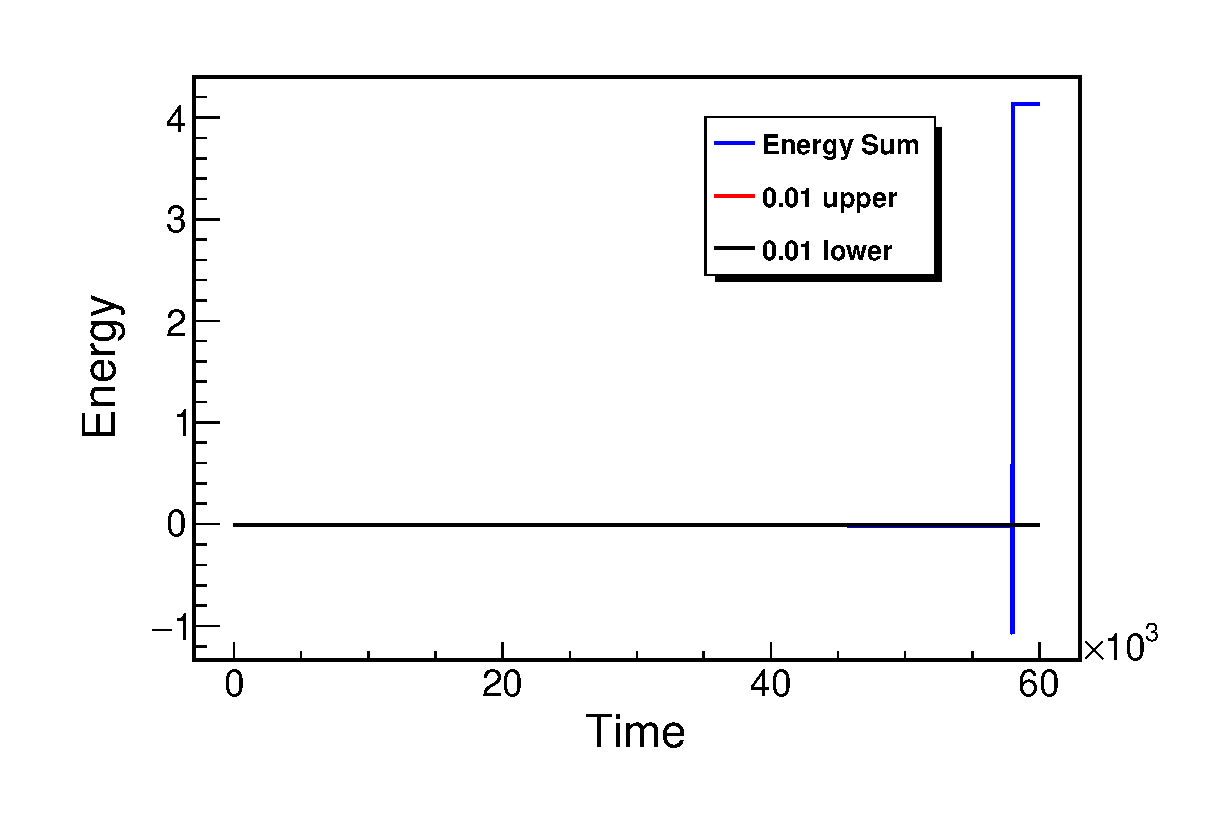
\includegraphics[width=0.5\textwidth]{figures/2ee.eps}}\\
\hfill
  \caption{\label{fig2} Plots for part 2. Top pane shows the three trajectories of the planets. The energy spectrum near the end of the simulation blows up as one of the planet is ejected out of a bound orbit.}
\end{figure}
One of the planets is ejected from an initially bound orbit via two interactions with the second planet, and a fatal interaction with the massive sun. The total energy of the system explodes in the final steps.
\subsection{Part 3}
d

\section{Problem 2 - LArgon}
\end{document}
